\documentclass{article}
\usepackage{graphicx}
\usepackage{times}
\usepackage{hyperref}
\usepackage{caption}
\usepackage{multirow}

\title{Big Data Final Ödevi}
\author{Ramazan Erduran}
\date{May 2023}

\begin{document}

\begin{titlepage}
    \begin{center}
        \centering
        
\includegraphics[width=0.4\textwidth]{Images/hacettepe_logo.png}
        
        \vspace*{1cm}
        \Huge
        \textbf{Büyük Veri Analitiği Final Ödevi}
        
        \vspace{2.5cm}
        
        \textbf{Ramazan Erduran}

        \Large
        21821809
        
        \vfill
        
        \Large
        İstatistik \\
        Hacettepe Üniversitesi \\
        30.05.2023
        
    \end{center}
\end{titlepage}

\clearpage
\tableofcontents

\clearpage
\section{Giriş}
Her geçen gün üretilen bilgi miktarı bir önceki güne kıyasla daha hızlı bir şekilde artmış ve bu nedenle bu büyük verileri analiz edip anlamlı içgörüler çıkarmak giderek daha önemli hale gelmiştir.

\vspace{5pt}
Büyük veri analitiği alanı, bu devasa veri havuzlarından anlamak, sınıflandırmak, analiz etmek, tahminlemeler yapmak ve değerli bilgiler çıkarmak gibi pek çok yöntemi kapsar. Ayrıca, bu alanda, araştırmacıların sofistike büyük veri analiz faaliyetleri uygulamalarını sağlamak için pek çok büyük veri işleme teknolojilerini kullanılır. KNIME'da bu teknolojilerden biridir.

\vspace{5pt}
Büyük veri faaliyetleri, ön işleme fonksiyonları, modelleme aktiviteleri ve öngörü işlemleri vb. şeyleri içerir. 

\vspace{5pt}
Bu raporlamada büyük veri analitiğiyle ilişkili temel kavramları aydınlatmayı ve aynı zamanda bir büyük veri analitiği uygulamasında KNIME'ın nasıl kullanılabileceğini göstermeyi amaçlıyorum.

\clearpage
\section{Büyük Veri ve İstatistik}
Açıkcası bu kısımda büyük veri ile istatistiği birbirinden ayırmak biraz tuhaf olacaktır. Zira büyük veri analitiğinde kullanılan tekniklerin belki de \%99'u istatistik temelli tekniklerdir.

\vspace{5pt}
Günümüzde karmaşık bilgilerin muazzam bir hacimle biriktirilmesi ve işlenmeye çalışılması, geleneksel hesaplama sistemlerinin etkin bir şekilde başa çıkamadığı bir seviyededir. İşte tam da burada büyük veri işlemede kullanılan teknolojiler devreye girer. Büyük veri, geleneksel veri işleme teknikleriyle kolayca yönetilemeyen yapılandırılmış ve yapılandırılmamış verilerdir. Öte yandan istatistik, veri toplama, analiz etme, yorumlama ve iç görüler üretmeye odaklı matematiksel bir daldır. 

\vspace{5pt}
Büyük veri ve istatistik benzer konuları ele alsa da, veri ölçeğinde, veri türlerinde ve uygulanan metodolojide farklılıklar gösterir. Büyük veri, gelişmiş hesaplama çerçeveleri aracılığıyla yüksek ölçekte verilerin analizi ve yönetimine odaklanırken, istatistik daha küçük çaplı veri setleri ile alakadardır. Zaten istatistiğin temelinde olasılıkları ve kitaleyi en iyi temsil eden örneklemi ele alarak daha küçük veri setleriyle daha büyük veri setleri hakkında yargılara varmaya çalışmak vardır. İstatistikte örnekleme yöntemleri ve hipotez testleri kullanılırken, büyük veri analitiğinde zaten kitlenin kendisi analiz edilmeye çalışıldığından hipotez kurmaya veya örneklem çekmeye gerek yoktur. 

\vspace{5pt}
Ancak bu farklılıklara rağmen büyük veri analitiği ve istatistik iç içe geçmiş alanlardır. Zira büyük veri analitiği ile elde edilen çıkarımlar istatistiksel teknikler ile yoğrularak daha doğru ve iyi kararlar almayı, veri kümelerini derinlemesine anlamayı sağlar.

\clearpage
\section{Veri Kümesi}
Uygulamada kullanılan veri kümesi Avrupa'daki bir bankadan (ismi belirtilmiyor) alınmıştır. Veri seti bankaya kayıtlı müşterilerin churn edip etmeyeceğine ilişkin verileri taşımaktadır.

Veri setinde bulunan değişkenlere ilişkin açıklamaya Tablo \ref{metadata}'te görüntülenmektedir.

\begin{table}[h]
    \caption{Meta}
    \label{metadata}
    \begin{tabular}{|c|c|}
        \hline
        \textbf{Değişken} & \textbf{Açıklaması} \\
        \hline
        RowNumber & Kayıt (sıra) numarasına karşılık gelir.\\
        \hline
        CustomerId & Müşteriye ait benzersiz bir değerdir. Her müşterininki farklıdır. \\
        \hline
        Surname & Müşterinin soyadı \\
        \hline
        CreditScore & Müşterinin kredi puanı \\
        \hline
        Geography & Müşterinin yaşadığı yeri belirtir. \\
        \hline
        Gender & Müşterinin cinsiyetini belirtir. \\
        \hline
        Age & Müşterinin yaşını belirtir. \\
        \hline
        Tenure & Müşterinin bankanın müşterisi olduğu yıl sayısını ifade eder. \\
        \hline
        Balance & Müşterinin hesap dengesini belirtir. \\
        \hline
        NumOfProducts & Bir müşterinin banka aracılığıyla satın aldığı ürün sayısını ifade eder. \\
        \hline
        HasCrCard & Müşterinin kredi kartı olup olmadığını gösterir. \\
        \hline
        IsActiveMember & Müşterinin aktif olup olmadığını gösterir. \\
        \hline
        EstimatedSalary & Müşterinin tahmini maaşını gösterir. \\
        \hline
        Complain & Müşterinin şikayetinin olup olmadığını gösterir. \\
        \hline
        SatisfactionScore & Müşterinin tatminiyet skorunu gösterir. \\
        \hline
        CardType & Müşterinin sahip olduğu kart tipini gösterir. \\
        \hline
        PointsEarned & Müşterinin kredi kartıyla topladığı puanı gösterir. \\
        \hline
        Exited & Müşterinin churn edip etmediğini gösterir (hedef değişken). \\
        \hline
    \end{tabular}
\end{table}

\vspace{10pt}
Bilindiği üzere bankaya yeni müşteri katmaktansa eldeki müşterilerin bankadan ayrılmasını engellemek daha az maaliyetli ve daha az yorucu bir iştir. Ayrıca eldeki müşterilerin memnuniyeti sağlandığında bankayı önerme olasılıkları artar ve dolaylı yoldan yeni müşteriler de elde etmiş oluruz. Bu amaçla hangi müşterilerin bankadan ayrılacağına ilişkin bir makine öğrenmesi projesi ile tahminlerde bulunacağız. Bankadan ayrılacak müşterilere ilişkin promosyon önerileri gibi önerilerde bulunulabilir...


\clearpage
\section{Uygulama}
\subsection{Verilerin Keşfi}
Verileri keşfetme sürecinde çeşitli görselleştirilmeler ile veri seti içerisinde gizli ilişkiler ve hedef değişkene olan etkiler araştırıldı.

Çıkarımlar şu şekilde elde edildi:
\begin{enumerate}
    \item Bankadan ayrılan müşterilerin çoğunluğunu kadınlar oluşturdu. 
    \item Bankadan ayrılan müşterilerin çoğunluğunu kadınlar oluşturdu. 
    \item Bankadan ayrılan müşterilerin konumlarına bakıldığında Almanya ve Fransa topluluğun \%40'ını oluştururken churn eden müşterilerin en azı İspanya'da bulunanlar oldu.
    \item İspanya'daki müşterilere ayrıcalık mı tanınıyor şeklinde bir inceleme yapıldı ve üç ülkenin de ortalama tatmin skoru eşit bulundu.
    \item Bankadan ayrılan müşterilerin tatmin skorlarında bir ilişki bulunamadı. Ayrılan ve ayrılmayan müşterilerin skorlarının ortalamaları 3 olarak bulundu. Demek ki müşterilerin gitmesine sebep olan farklı bir durum var, zira tatmin skorları 3/5 olarak bulundu.
\end{enumerate}

\subsection{İlişkisel Veri Analizi}
Değişkenlerin birbiri ile olan ilişkileri incelendi ve sonuçlar şu şekilde elde edildi:
\begin{enumerate}
    \item Bağımsız değişkenlerin kendi aralarındaki ilişkileri incelendiğinde sadece \textit{ürün sayısı} ile \textit{hesap bakiyesi} değişkenleri arasında orta düzeyde doğrusal ilişki bulundu. 
    Diğer değişkenlerin birbiri ile ilişkisi çok zayıf ya da yok olarak belirlendi.
    \item Müşterinin bankadan ayrılıp ayrılmadığını belirten, hedef değişken olan \textit{churn} değişkeni üzerindeki ilişkileri incelendiğinde en çok etkisi olan değişken \textit{\textbf{şikayet}} değişkeni old. Öyle ki karar ağaçları algoritmasında bu değişkenin veri setine eklenmesi ile başarı oranı \%100'e ulaştı.
    Bu nedenle bu değişkeni veri setinden çıkarıp daha gerçek dünyaya uygulanabilir bir veri setiymişcesine işlemler yapılmaya devam edildi.
    \item Hedef değişkenle olan ilişkilerin yanı sıra bağımsız değişkenler için PCA (Temel Bileşenler Analizi) yapılmak istendi ancak bağımsız değişkenlerin kendi içlerindeki çok zayıf/yok derecesindeki korelasyondan dolayı bu işleme devam edilemedi.
\end{enumerate}

Yukarıdaki sonuçlardan hareketle veri setine dair tüm çıkarımların yapıldığı sonucuna varılıp makine öğrenmesi adımına geçildi.

\subsection{Tahmin Yapma Aşaması}
Tahmin aşamasına gelindiğinde sınıflandırma algoritmaları olarak:
\begin{itemize}
    \item Karar Ağaçları Algoritması
    \item Lineer Regresyon Algoritması
    \item En Yakın Komşu Algoritması
\end{itemize}
Kullanıldı.

Algoritmaların sonuçları değerlendirilirken iki adet metrik kullanıldı. Bu metrikler yüzdelik doğruluk oranı (Accuracy) ve Kappa katsayısı oldu. Kullanılan metriklere göre en iyi sonucu veren algoritma lojistik regresyon oldu.

\textit{Şikayet} değişkeni modeldeyken \%100 doğruluk ile en iyi sonucu veren model karar ağaçları algoritmasıyken bu değişkeni veri setinden çıkardığımızda en iyi sonucu veren algoritma lojistik regresyon oldu.

Değişkenin modelden çıkarılması hususunda:

\begin{figure}[htbp]
    \centering
    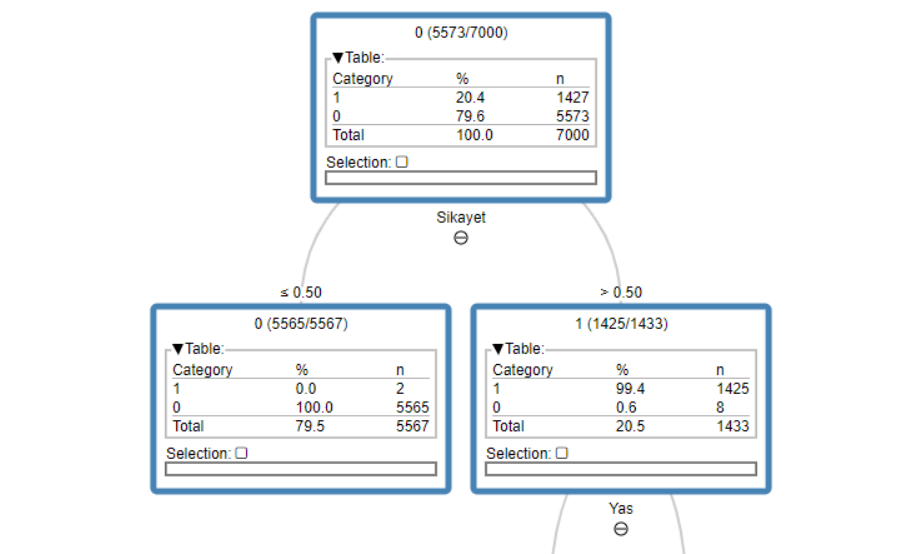
\includegraphics[width=0.8\textwidth]{Images/dt1.png}
    \caption{Şikayet değişkeni modeldeyken}
    \label{Karar Ağaçları 1}
\end{figure}

\ref{Karar Ağaçları 1} Numaralı resimde de görüldüğü üzere şikayeti 0.50'nin altındaki kişiler gerçekten de churn etmemiş ve buradaki oran \%79.5 olarak belirtilmiş. Geriye kalan \%21.5'luk veriyi de kolay bir şekilde dallandırarak \%100'lük bir başarıya ulaşmış. Ancak bu durum gerçek hayatı yansıtmayacağından ilgili değişken veri setinden çıkarılıp tekrar denendiğinde ise \ref{Karar Ağaçları 2}'de bulunan sonuçlar elde edildi.
\clearpage

\begin{figure}[htbp]
    \centering
    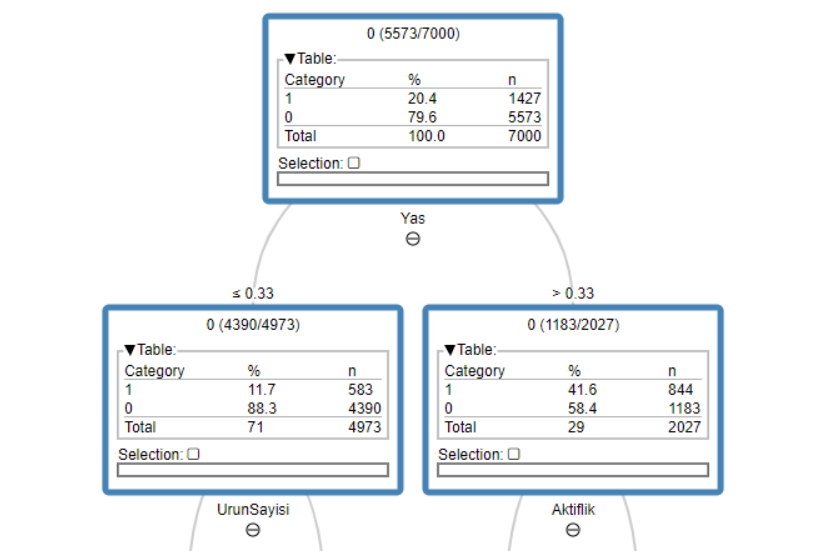
\includegraphics[width=0.8\textwidth]{Images/dt2.png}
    \caption{Şikayet değişkeni modelden çıkarıldığında}
    \label{Karar Ağaçları 2}
\end{figure}

\ref{Karar Ağaçları 2} Numaralı resimde de görüldüğü üzere artık model \%100'lük bir doğruluktan ziyade daha normal, kabul edilebilir, gerçek dünyaya uygun şekilde tahmin yapmakta.

Tüm bu yorumlamalardan sonra en nihayetinde \textit{Şikayet} değişkeni veri setinden çıkarıldı ve 3 farklı model denendi. En iyi model ise lojistik regresyon modeli oldu.

Modele hiper parametre ayarı da yapıldı ve en iyi modelin hiper parametreleri;
\begin{enumerate}
    \item Solver: Iteratively reweighted least squares 
\end{enumerate}
Şeklinde elde edildi.

\clearpage
\section{Sonuç ve Tartışma}
Sonuç olarak veri ön işleme, veri görselleştirme ve bu görselleştirmelerden içgörü elde etme, keşifsel ve ilişkisel veri analizi yapma, makine öğrenmesi ile tahminlerde bulunma, modelleri çeşitli metriklerle değerlendirme ve sonucunda hipoer parametre ayarı ile en iyi modeli bulma adımları tamamlandı.

Bu adımların sonucunda müşterilerin bankadan ayrılmasını en çok etkileyen değişken \textbf{şikayet} değişkeni olurken en iyi tahmin modeli (\textbf{şikayet} değişkeni veri setinde değilken) lojistik regresyon modeli oldu.

Modellerin değerlendirme süreçlerine ilişkin sonuçlar Tablo \ref{tab:acc}'te görülebilir

\vspace{10pt}
\begin{table}[h]
    \centering
    \caption{Değerlendirme Sonuçları}
    \begin{tabular}{|c|c|c|}
         \hline
         \multirow{2}{*}{\textbf{Model}} & \multicolumn{2}{c|}{\textbf{Metrikler}} \\
         \cline{2-3}
         & \textbf{Accuracy} & \textbf{Kappa} \\
         \hline
         Decision Tree & \%80.167 & 0.373 \\
         Lojistik Regresyon & \%80.733 & 0.206 \\
         KNN & \%78.267 & 0.187 \\
         \hline
    \end{tabular}
    \label{tab:acc}
\end{table}

Değerlendirme sonucu en iyi olan lojistik regresyon modelinin hipoer parametre ayarı yapıldıktan sonra \%81.467 accuracy ve 0.245 kappa sayısına sahip oldu.

\clearpage
\section{Kaynakça}
\begin{enumerate}
    \item Berthold, M. R., Cebron, N., Dill, F., Gabriel, T. R., Kötter, T., Meinl, T., \& Sieb, C. (2008). KNIME: The Konstanz Information Miner. Data Mining and Knowledge Discovery Handbook, 1-17.
    \item Chen, H., Chiang, R. H. L., \& Storey, V. C. (2012). Business intelligence and analytics: From big data to big impact. MIS quarterly, 36(4), 1165-1188.
    \item KNIME Hub: \href{https://hub.knime.com/}{https://hub.knime.com/}
    \item Statology: \href{https://www.statology.org/}{https://www.statology.org/}
\end{enumerate}


\end{document}
